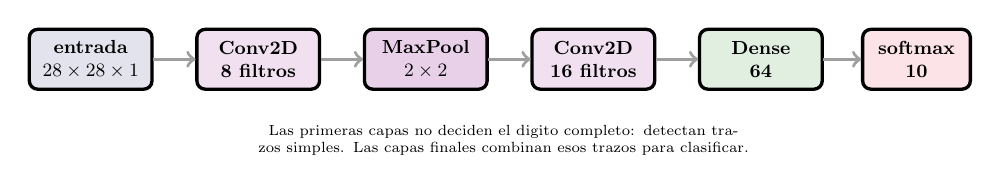
\begin{tikzpicture}[scale=0.76,transform shape]
\tikzstyle{box}=[draw,rounded corners=3pt,very thick,minimum width=2.05cm,minimum height=1.0cm,align=center,font=\small\bfseries]
\node[box,fill=MidnightBlue!12] (input) at (0,0) {entrada\\$28\times28\times1$};
\node[box,fill=Purple!12] (conv1) at (2.8,0) {Conv2D\\8 filtros};
\node[box,fill=Purple!18] (pool1) at (5.6,0) {MaxPool\\$2\times2$};
\node[box,fill=Purple!12] (conv2) at (8.4,0) {Conv2D\\16 filtros};
\node[box,fill=ForestGreen!14] (dense) at (11.2,0) {Dense\\64};
\node[box,fill=Crimson!12,minimum width=1.8cm] (out) at (13.8,0) {softmax\\10};
\foreach \a/\b in {input/conv1,conv1/pool1,pool1/conv2,conv2/dense,dense/out} {
  \draw[->,very thick,gray!75] (\a) -- (\b);
}
\node[font=\scriptsize,align=center,text width=12.0cm] at (6.9,-1.35) {Las primeras capas no deciden el digito completo: detectan trazos simples. Las capas finales combinan esos trazos para clasificar.};
\end{tikzpicture}
